% Created 2021-11-12 Fri 23:20
% Intended LaTeX compiler: pdflatex
\documentclass{scrartcl}
\usepackage[utf8]{inputenc}
\usepackage[T1]{fontenc}
\usepackage{fontspec}
\usepackage{graphicx}
\usepackage{grffile}
\usepackage{longtable}
\usepackage{wrapfig}
\usepackage{rotating}
\usepackage[normalem]{ulem}
\usepackage{amsmath}
\usepackage{textcomp}
\usepackage{amssymb}
\usepackage{capt-of}
\usepackage[dvipsnames]{xcolor}
\usepackage[colorlinks=true, linkcolor=Blue, citecolor=BrickRed, urlcolor=PineGreen]{hyperref}
\usepackage{indentfirst}
% features: (custom-font acronym underline par-sep alegreya-typeface image)
\usepackage[osf]{Alegreya}
\usepackage{AlegreyaSans}
\usepackage[scale=0.88]{sourcecodepro}

\newcommand{\acr}[1]{\protect\textls*[110]{\scshape #1}}
\newcommand{\acrs}{\protect\scalebox{.91}[.84]\hspace{0.15ex}s}
\usepackage[normalem]{ulem}
\setlength{\parskip}{\baselineskip}
\setlength{\parindent}{0pt}

\usepackage{graphicx}
% end features
\author{Shaurya Singh}
\date{\today}
\title{IRR 1}
\colorlet{greenyblue}{blue!70!green}
\colorlet{blueygreen}{blue!40!green}
\providecolor{link}{named}{greenyblue}
\providecolor{cite}{named}{blueygreen}
\hypersetup{
  pdfauthor={Shaurya Singh},
  pdftitle={IRR 1},
  pdfkeywords={},
  pdfsubject={},
  pdfcreator={Emacs 29.0.50 (Org mode 9.6)},
  pdflang={English},
  breaklinks=true,
  colorlinks=true,
  linkcolor=,
  urlcolor=link,
  citecolor=cite
}
\urlstyle{same}
\usepackage[notquote]{hanging}
\begin{document}\makeatletter
\newcommand{\citeprocitem}[2]{\hyper@linkstart{cite}{citeproc_bib_item_#1}#2\hyper@linkend}
\makeatother



\maketitle

\section*{Introduction}
\label{sec:org532d088}
Diabetes is becoming one of the most widespread health-burning problems in the middle-aged and elderly. The worldwide prevalence of diabetes among subjects over 65 years was 135.6 million in 2019, a number that is expected to double in 2045 (\citeprocitem{8}{Sinclair et al. 2020}). More than 150 million Americans account for 140 billion cups of consumed coffee per year. Nearly four in 10 American teens drink coffee. Caffeine intake in teenagers has exponentially grown since 2004, yet it has gone largely unnoticed. However, growing concerns over the adverse health effects of caffeine suggest a comprehensive study. Previous studies have shown a link between adolescent coffee consumption and a decrease in the rate of middle-aged type 2 diabetes in those subjects (\citeprocitem{1}{ALPERET et al. 2019}). In a double-blind randomized trial, coffee intake was shown to decrease fat mass in healthy overweight adults, suggesting coffee could be modulating lower type 2 diabetes mellitus(T2DM) risk among adults, but research done by the National Health Research Institute of Taiwan states otherwise. The institute believes the ease of access to Sugar-Sweetened-Beverages (SSB’s) such as coffee and tea in Taiwan have caused an increase in adolescent obesity, diabetes, and resulted in less satisfactory health overall (\citeprocitem{6}{Lin et al. 2011}), which prompts us: what is the influence of adolescent coffee consumption and coffee culture on future risk of type 2 diabetes mellitus in middle-aged men and women?

\section*{Caffeine Addiction and its Effect on Our World}
\label{sec:org398c9f7}
Caffeine is now the most commonly used drug in the world (\citeprocitem{4}{Gilbert 1984}). Although caffeine consumed in moderation is generally safe, an increasing number of clinical studies are showing how easy it is to get addicted. Users dependant on the drug are often unable to reduce their consumption, despite knowing the recurring health problems and consequence of excess caffeine and sugar consumption. The WHO now recognizes caffeine dependence as a clinical disorder, as caffeine use in excess can result in serious health hazards and in rare cases even death (\citeprocitem{2}{Brockwell, Eikelboom, and Beninger 1991}).

Unlike other drugs, caffeine is legal, easy to obtain, and socially acceptable to consume. Although before the mid 2000's caffeinated beverages were generally used by adults, such drinks are now consumed regularly by children. Additionally, these caffeinated drinks are specifically marketed to children, some as young as 5 years of age. Historically, soda and tea have been the main sources of caffeine in the diets of children and adolescents; however, the availability and sales of energy drinks, coffee drinks, and food products containing caffeine have dramatically increased over the past decade and are often marketed toward children and adolescents (\citeprocitem{5}{Heckman, Sherry, and De Mejia 2010}). In addition, the caffeine content of energy drinks is not currently regulated by the FDA because the former are marketed as and considered dietary supplements (\citeprocitem{5}{Heckman, Sherry, and De Mejia 2010}). Excess consumption of caffeine can result in tachycardia, arrhythmia, hypertension, hyperactivity, anxiety, and increased blood sugar concentrations because many energy drinks, coffee drinks, and other drinks that contain large amounts of caffeine often also contain high amounts of sugar (\citeprocitem{7}{Seifert et al. 2011}).

\section*{The Growing Worldwide Prevalence of Diabetes}
\label{sec:orgee47729}
Diabetes millitus is a chronic metabolic disorder, characterized by persistent hyperglycemia. Its often linked to impaired insulin secretion, resistance to peripheral actinos of insulin, or both. According to the International Diabetes Federation (IDF), approximately 415 million adults between the ages of 20 to 79 years had diabetes mellitus in 2015 (\citeprocitem{11}{Zheng, Ley, and Hu 2017}). DM is proving to be a global public health burden as this number is expected to rise to another 200 million by 2040 (\citeprocitem{11}{Zheng, Ley, and Hu 2017}). Chronic hyperglycemia in synergy with the other metabolic aberrations in patients with diabetes mellitus can cause damage to various organ systems, leading to the development of disabling and life-threatening health complications, most prominent of which are microvascular (retinopathy, nephropathy, and neuropathy).

The association between coffee consumption and risk of some chronic diseases including cardiovascular disease and cancer has been reported (\citeprocitem{3}{Dam 2008}). Several recent studies reported that coffee consumption is inversely related to the risk of type 2 diabetes (\citeprocitem{9}{Tuomilehto et al. 2004}). Different components in coffee such as antioxidants, phenol chlorogenic acid, magnesium, and caffeine have been proposed to be involved in the process of developing type 2 diabetes (\citeprocitem{10}{Van Dam and Hu 2005}).

\begin{center}
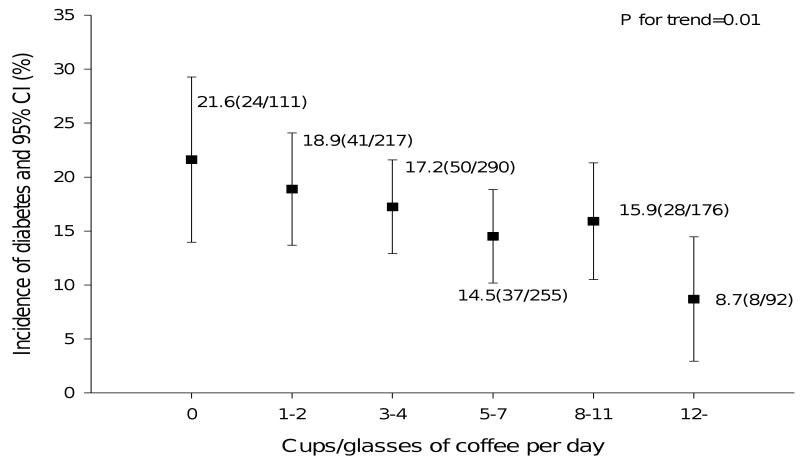
\includegraphics[width=.9\linewidth]{/Users/shauryasingh/org/.attach/57/bc0be2-0dc2-4cbb-8c47-4ed807c83352/_20211112_222930nihms160871f1.jpg}
\end{center}


\section*{References}
\label{sec:org43bbf69}
\begin{hangparas}{1.5em}{1}
\hypertarget{citeproc_bib_item_1}{ALPERET, DERRICK, KLODIAN DHANA, JORGE E. CHAVARRO, and QI SUN. 2019. “1575-P: Influence of Adolescent and Maternal Coffee Consumption on Risk of Obesity and Type 2 Diabetes Mellitus in Middle-Aged Women and Their Offspring: Results from Two Prospective Cohort Studies in the United States” 68 (Supplement 1): 1575–P. \href{https://doi.org/10.2337/db19-1575-p}{https://doi.org/10.2337/db19-1575-p}.}

\hypertarget{citeproc_bib_item_2}{Brockwell, Neil T, Roelof Eikelboom, and Richard J Beninger. 1991. “Caffeine-Induced Place and Taste Conditioning: Production of Dose-Dependent Preference and Aversion.” \textit{Pharmacology Biochemistry and Behavior} 38 (3): 513–17.}

\hypertarget{citeproc_bib_item_3}{Dam, Rob M van. 2008. “Coffee Consumption and Risk of Type 2 Diabetes, Cardiovascular Diseases, and Cancer.” \textit{Applied Physiology, Nutrition, and Metabolism} 33 (6): 1269–83.}

\hypertarget{citeproc_bib_item_4}{Gilbert, RM. 1984. “Caffeine Consumption. The Methylxanthine Beverages and Foods: Chemistry, Consumption, and Health Effects (Spiller GA Ed) Pp 185–213, Alan R. Liss.” \textit{Inc., New York}.}

\hypertarget{citeproc_bib_item_5}{Heckman, MA, Kendle Sherry, and E Gonzalez De Mejia. 2010. “Energy Drinks: An Assessment of Their Market Size, Consumer Demographics, Ingredient Profile, Functionality, and Regulations in the United States.” \textit{Comprehensive Reviews in Food Science and Food Safety} 9 (3): 303–17.}

\hypertarget{citeproc_bib_item_6}{Lin, Wen-Yuan, F. Xaiver Pi-Sunyer, Ching-Chu Chen, Lance E. Davidson, Chiu-Shong Liu, Tsai-Chung Li, Mei-Fong Wu, Chia-Ing Li, Walter Chen, and Cheng-Chieh Lin. 2011. “Coffee Consumption Is Inversely Associated with Type 2 Diabetes in Chinese” 41 (6): 659–66. \href{https://doi.org/10.1111/j.1365-2362.2010.02455.x}{https://doi.org/10.1111/j.1365-2362.2010.02455.x}.}

\hypertarget{citeproc_bib_item_7}{Seifert, Sara M, Judith L Schaechter, Eugene R Hershorin, and Steven E Lipshultz. 2011. “Health Effects of Energy Drinks on Children, Adolescents, and Young Adults.” \textit{Pediatrics} 127 (3): 511–28.}

\hypertarget{citeproc_bib_item_8}{Sinclair, Alan, Pouya Saeedi, Abha Kaundal, Suvi Karuranga, Belma Malanda, and Rhys Williams. 2020. “Diabetes and Global Ageing among 65\textendash99-Year-Old Adults: Findings from the International Diabetes Federation Diabetes Atlas, 9th Edition” 162 (April): 108078. \href{https://doi.org/10.1016/j.diabres.2020.108078}{https://doi.org/10.1016/j.diabres.2020.108078}.}

\hypertarget{citeproc_bib_item_9}{Tuomilehto, Jaakko, Gang Hu, Siamak Bidel, Jaana Lindström, and Pekka Jousilahti. 2004. “Coffee Consumption and Risk of Type 2 Diabetes Mellitus among Middle-Aged Finnish Men and Women.” \textit{Jama} 291 (10): 1213–19.}

\hypertarget{citeproc_bib_item_10}{Van Dam, Rob M, and Frank B Hu. 2005. “Coffee Consumption and Risk of Type 2 Diabetes: A Systematic Review.” \textit{Jama} 294 (1): 97–104.}

\hypertarget{citeproc_bib_item_11}{Zheng, Yan, Sylvia H. Ley, and Frank B. Hu. 2017. “Global Aetiology and Epidemiology of Type 2 Diabetes Mellitus and Its Complications” 14 (2): 88–98. \href{https://doi.org/10.1038/nrendo.2017.151}{https://doi.org/10.1038/nrendo.2017.151}.}
\end{hangparas}
\end{document}
